% Appendix B

\chapter{Figures} % Main appendix title

\label{AppendixB} % For referencing this appendix elsewhere, use \ref{AppendixA}

\lhead{Appendix B. \emph{Figures}} % This is for the header on each page - perhaps a shortened title

\begin{figure}[!ht]
\center
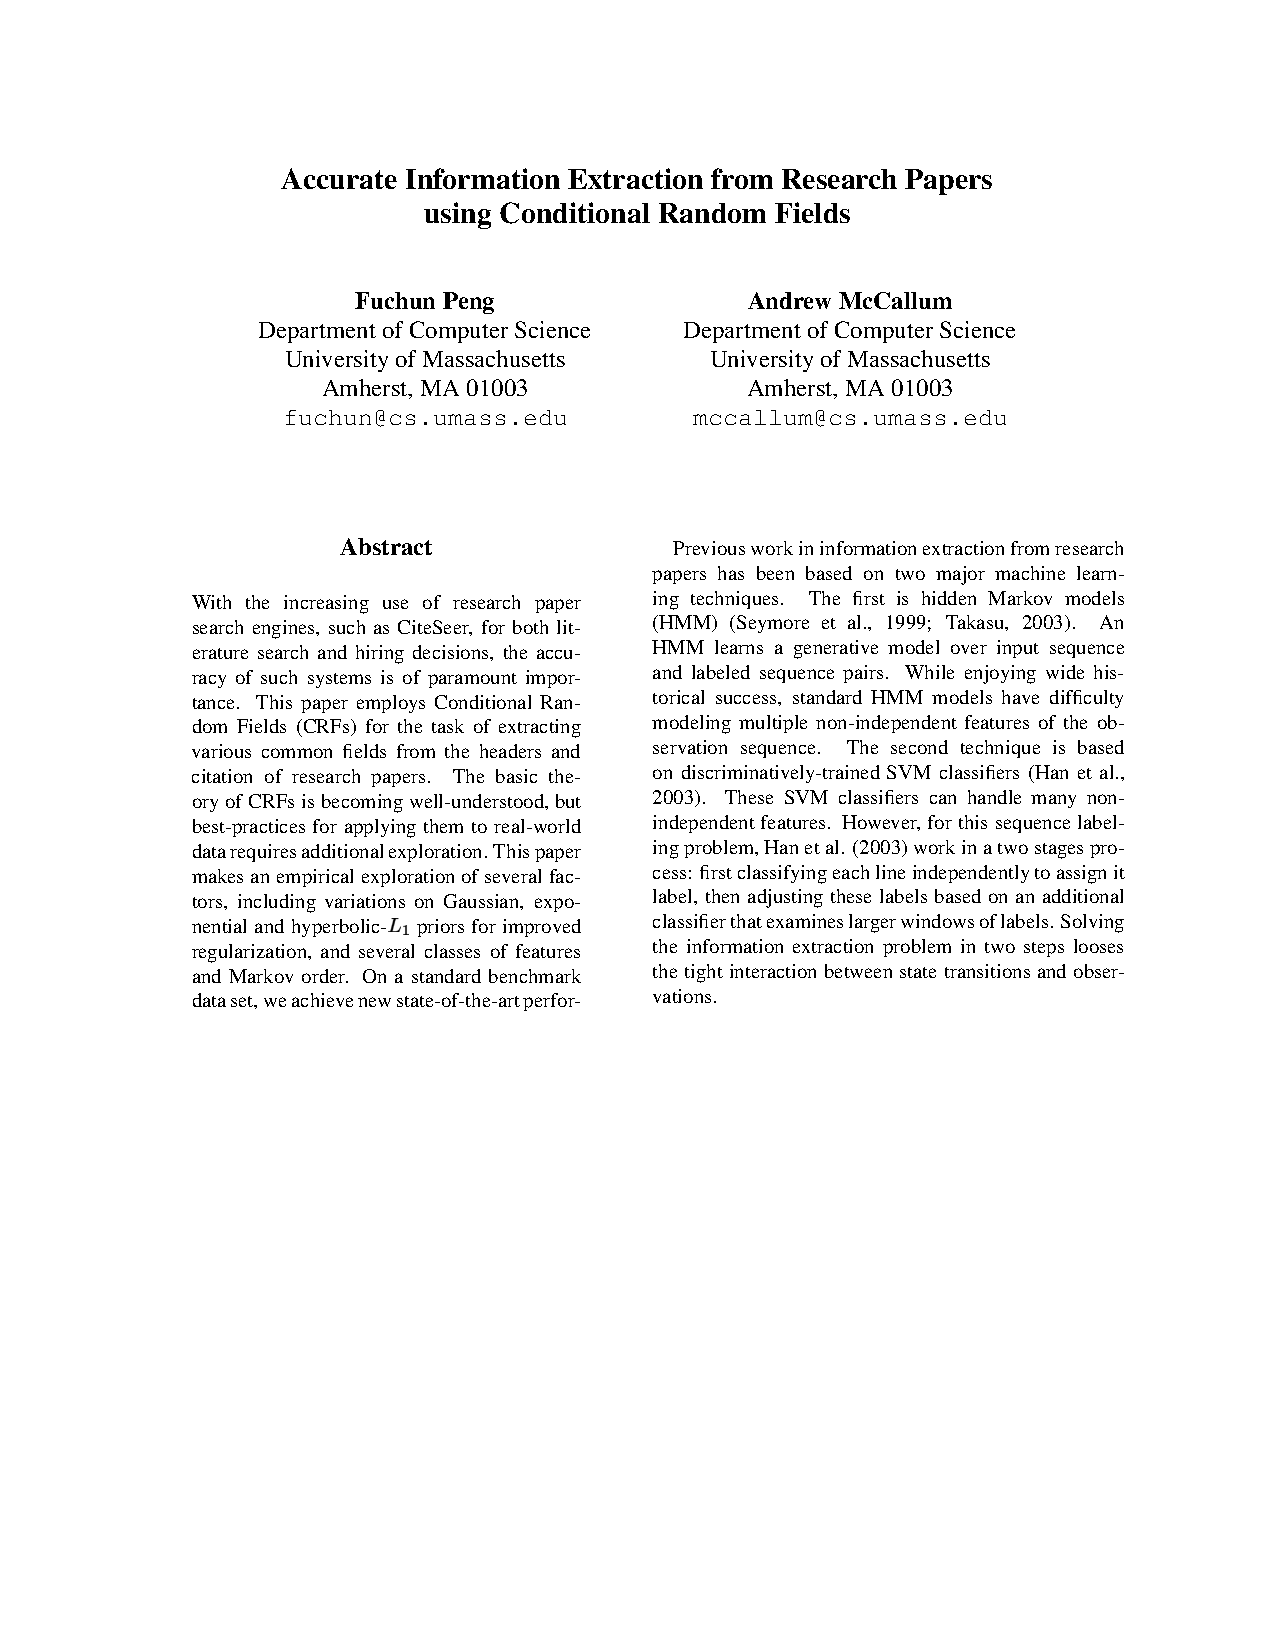
\includegraphics[width=3.25in]{Figures/header1.pdf}
\caption{The header section of a scientific paper. Excerpt from \cite{Peng04accurateinformation}}
\label{fig:header1}
\end{figure}

\begin{figure}[!ht]
\center
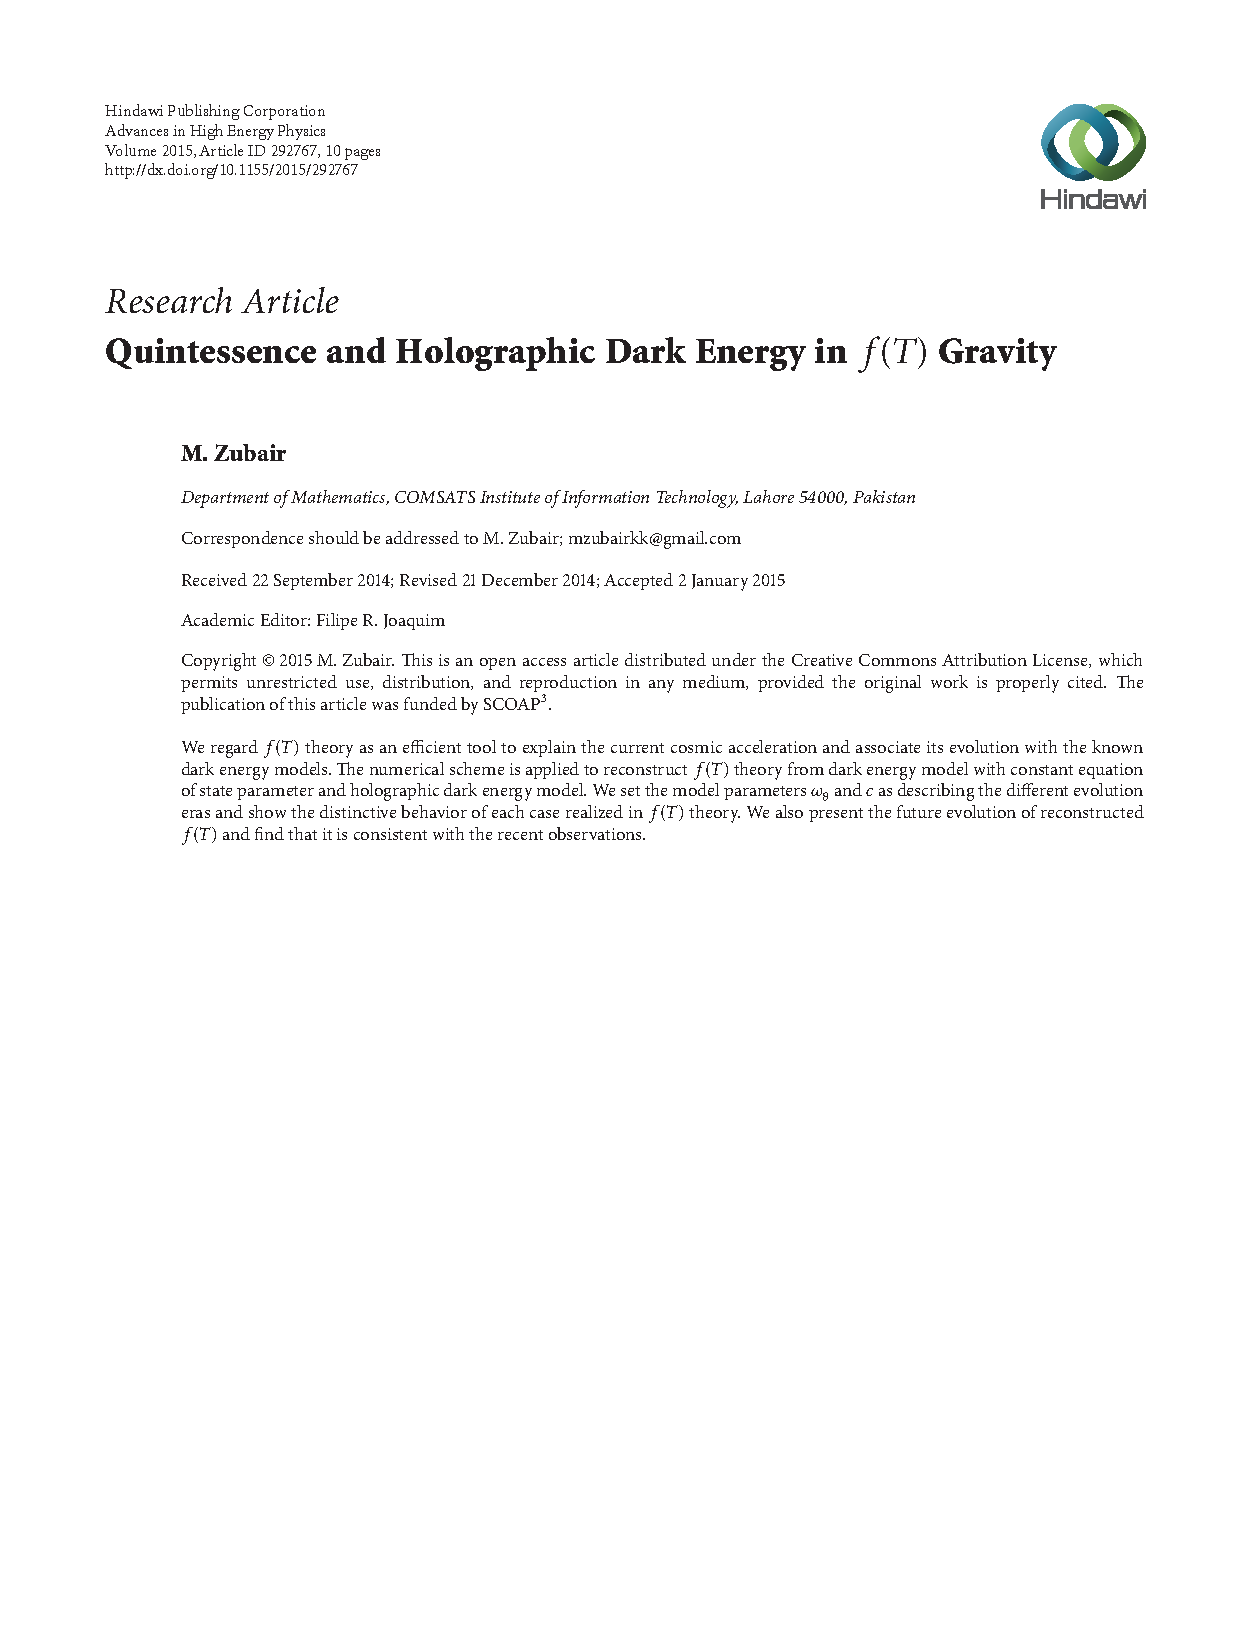
\includegraphics[width=3.25in]{Figures/header2.pdf}
\caption{The header section of a HEP paper. Excerpt from \cite{zubair2015quintessence}}
\label{fig:header2}
\end{figure}

\begin{figure}[h]
\center
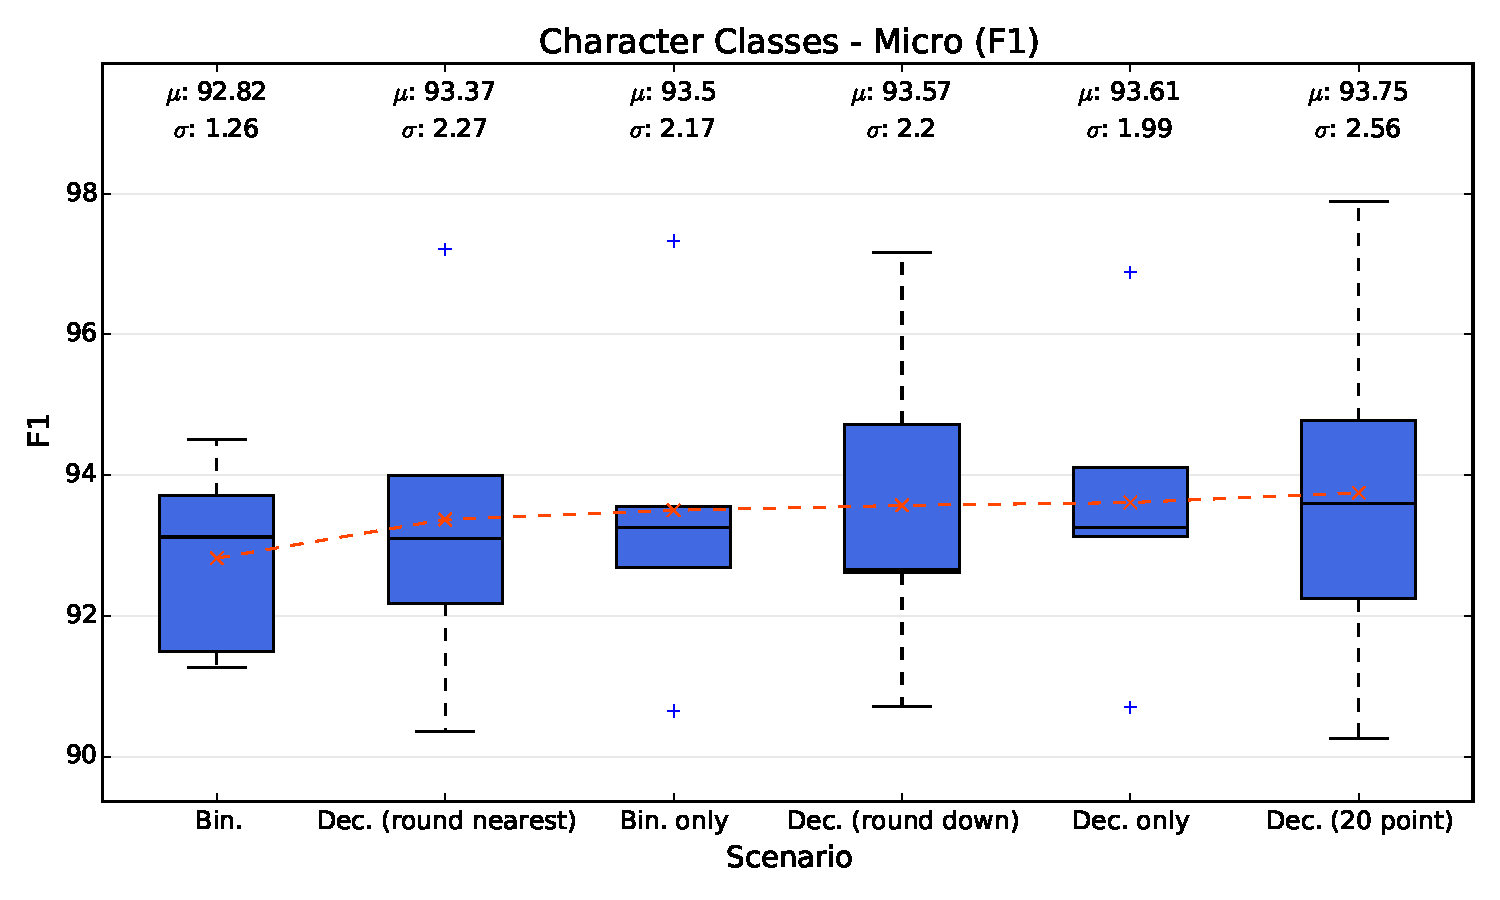
\includegraphics[width=5.5in]{Figures/micro_classes.pdf}
\caption{Comparison of different character class feature discretisation strategies.}
\label{fig:classes_micro}
\end{figure}

\begin{figure}[h]
\center
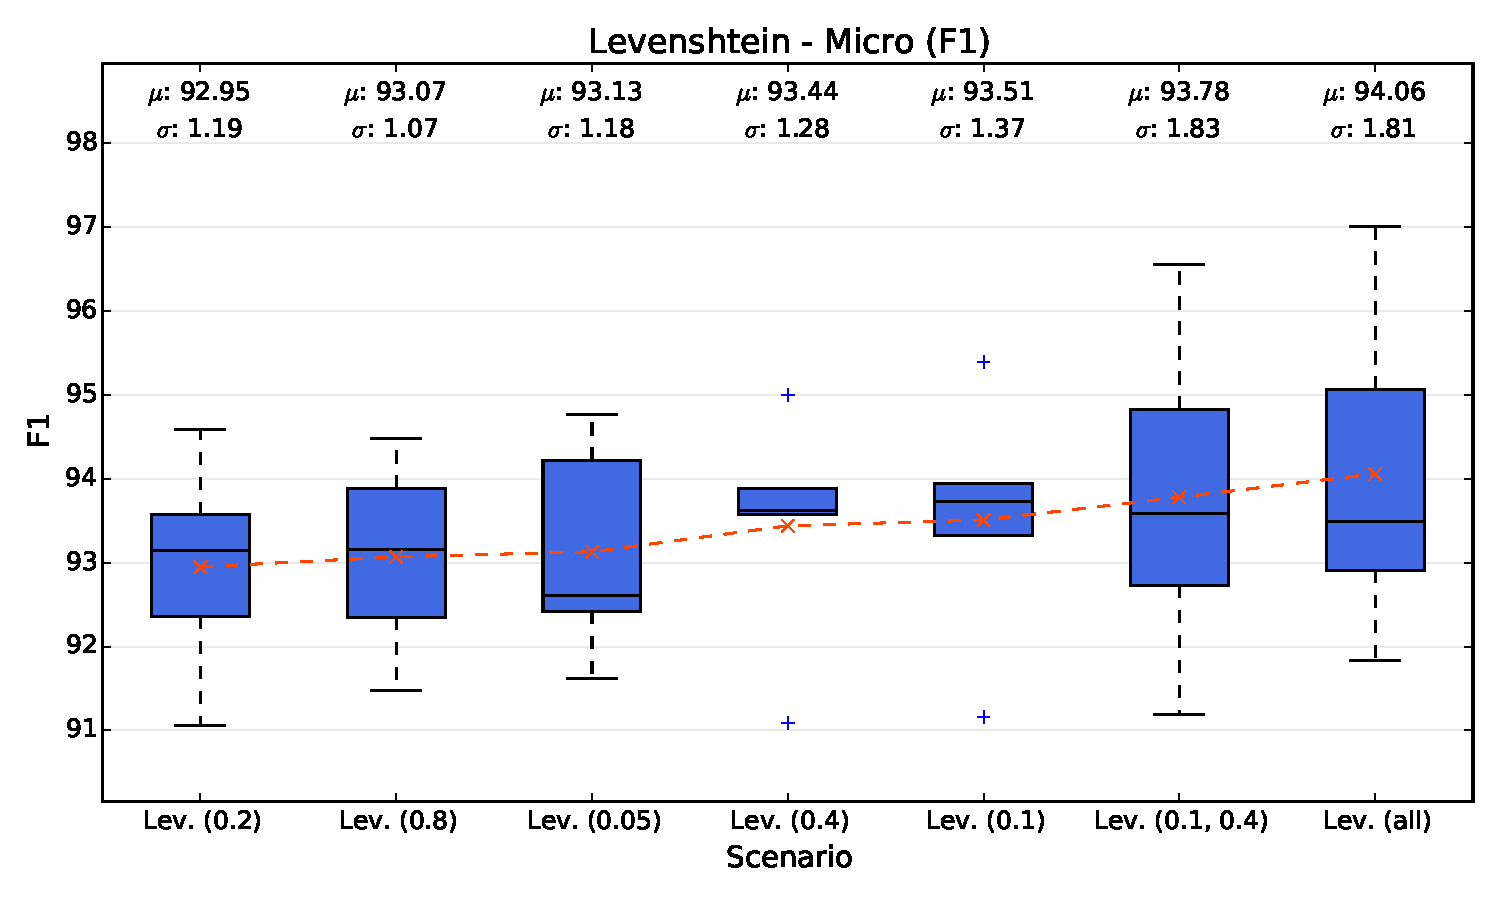
\includegraphics[width=5.5in]{Figures/micro_levenshtein.pdf}
\caption{Comparison of different levenshtein distance feature thresholding strategies.}
\label{fig:levenshtein_micro}
\end{figure}

\begin{figure}[h]
\center
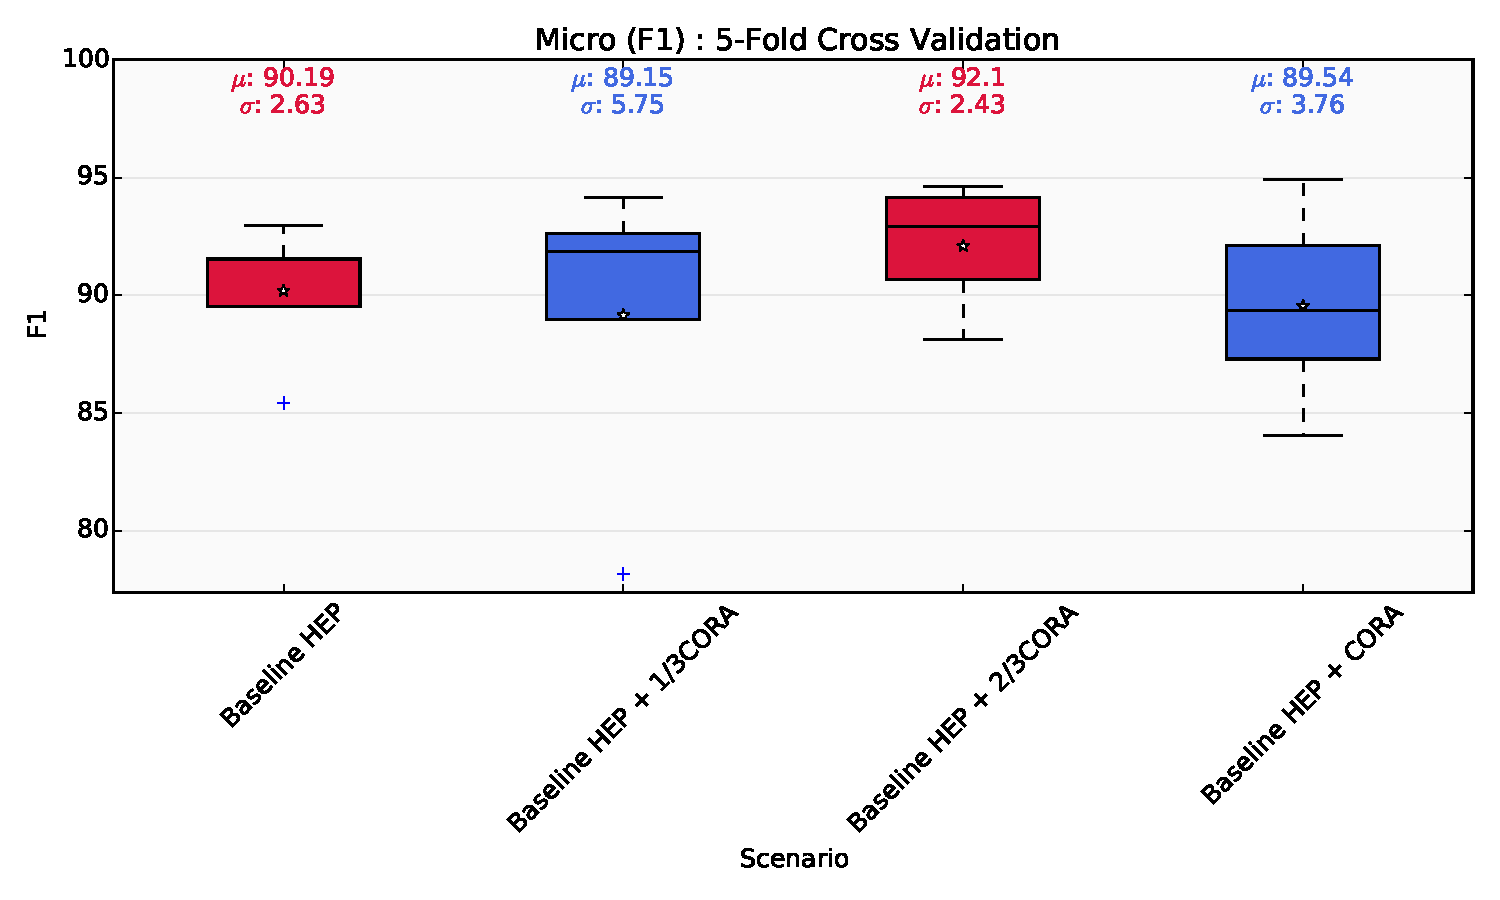
\includegraphics[width=5.5in]{Figures/micro_subsampling.pdf}
\caption{Comparison of different data configurations subsampling the CORA dataset.}
\label{fig:subsampling_micro}
\end{figure}

\begin{figure}[h]
\center
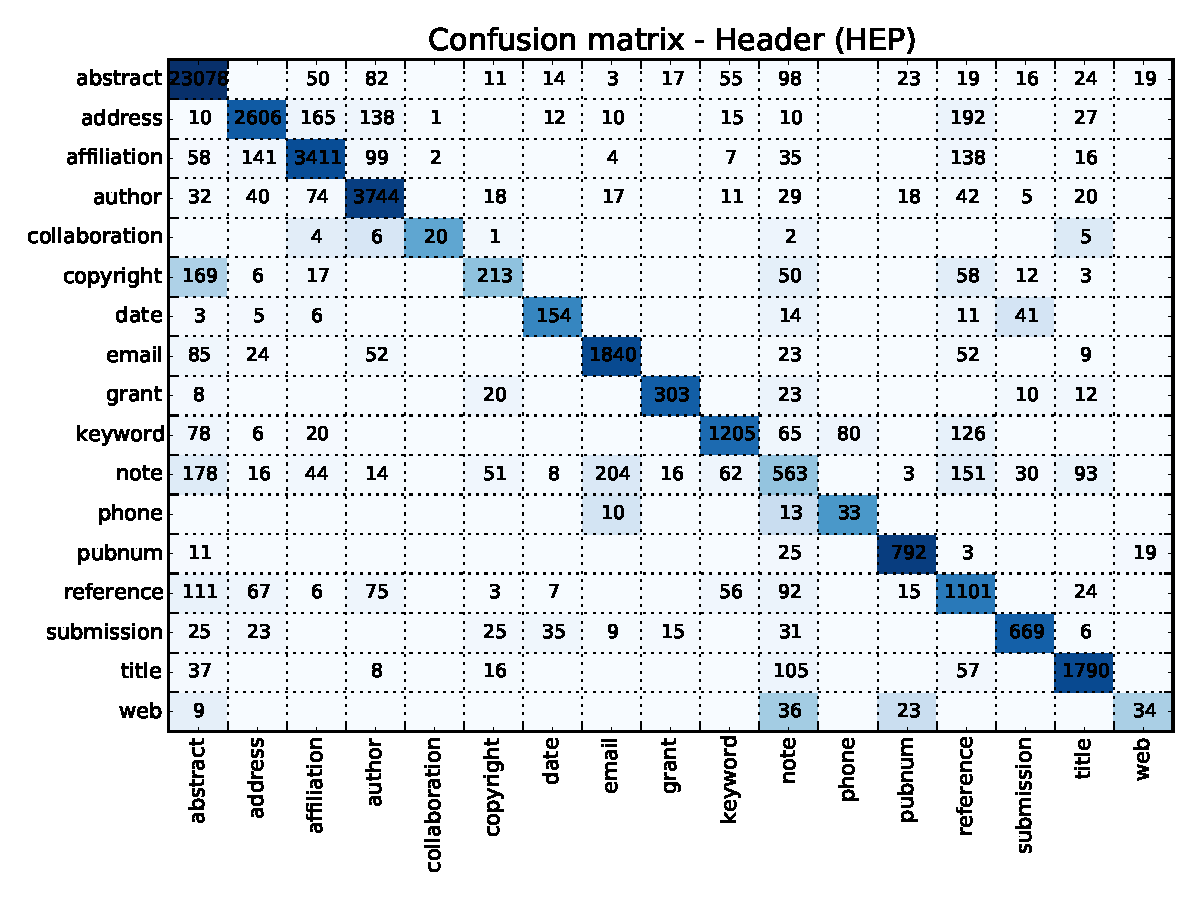
\includegraphics[width=5.5in]{Figures/baseline_confusion_header.pdf}
\caption{Confusion matrix for \emph{header} model, baseline features, trained on HEP data..}
\label{fig:confusion_header}
\end{figure}
